\begin{tikzpicture}[overlay, remember picture]
    \node[anchor=north west, rotate=0, gray, font=\tiny, text width=\paperwidth] at (current page.south west)  [xshift=0, yshift=0.75cm] {
    [1] L. Amico et al., Entanglement in Many-Body Systems, Reviews of Modern Physics 80, no. 2 (2008)
    };
\end{tikzpicture}


% \only<1>{
Some property, that differs for separable and entangled states.


\begin{figure}[h]
    \centering
    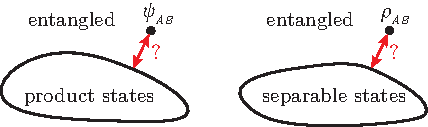
\includegraphics{imgs/Asset 2.pdf}
    %\caption{}
    %\label{fig:}
\end{figure}

% }

\onslide<2,3>{

\phantom{42}

A state $\rho_{AB}$ is entangled if and only if a positive map $\Lambda$ exists: 
\vspace{-2mm}
\begin{equation*}
	\left(\mathbbm{1}_A \otimes \Lambda_B \right) \rho_{AB} < 0.
\end{equation*}

}


\onslide<3>{

% \phantom{42}

Peres-Horodecki criterion of being separable:
\vspace{-2mm}
\begin{equation*}
	\rho_{AB}^{T_B} \geq 0.
\end{equation*}

}